%%
%% CONSISTENCY NOTIONS
%%
\section{Notions of Consistency and its Preservation}
\label{chap:correctness:notions_consistency}

We begin with a informal discussion of different ways to consider consistency. This especially involves \emph{intensional} and \emph{extensional} notions of consistency as well a \emph{monolithic} and \emph{modular} notions.


\subsection{Intensional and Extensional Consistency Notions}

\mnote{Intensional / extensional consistency}
When we consider a set of models, we would intuitively say that it is consistent if it fulfills some kind of constraints.
Defining these constraints to derive or check whether a given set of models is consistent constitutes an \emph{intensional specification} of consistency, because the set that contains all consistent models is intensionally represented by these constraints and can be derived from it.
We can consider a set of constraints as a predicate, i.e. a Boolean-valued function $I$, which indicates whether a model set $\modelset{m}$ fulfills the constraints $I: \metamodelsetinstanceset{M} \mapsto \setted{true, false}$. Then we can say that:
\begin{align*}
    \modelset{m} \consistenttomath I \equivalentperdefinition I(\modelset{m}) = true
\end{align*}
On the contrary, one can also enumerate the consistent sets of models, thus a set of models is considered consistent if it is contained in that enumeration.
This constitutes an \emph{extensional specification} of consistency.
Given such an enumeration $E = \setted{\modelset{m} \mid \modelset{m} \mathtext{is consistent}}$, we can say that:
\begin{align*}
    \modelset{m} \consistenttomath E \equivalentperdefinition \modelset{m} \in E
\end{align*}

\mnote{Equivalence intensional / extensional specifications}
It is easy to see that both kinds of specifications are equivalent. For each intensional specification the extensional one can be derived by enumerating all models that fulfill the constraints:
\begin{align*}
    E = \setted{\modelset{m} \mid I(\modelset{m}) = true}
\end{align*}
An extensional specification could also be transferred to an intensional one by defining constraints that are fulfilled by exactly the enumerated instances:
\begin{align*}
    I(\modelset{m}) \mapsto 
    \begin{cases} 
        true, & \modelset{m} \in E\\
        false, & \modelset{m} \not\in E\\
    \end{cases}
\end{align*}
For us, however, it will only be relevant that an intensional specification can be transformed into an extensional one.

\mnote{Extensional specifications for theoretical considerations}
A developer who defines consistency, usually wants to use an intensional specification, as tools like transformation languages usually allow the specification of constraints rather than enumerating consistent instances. This is due to the fact that he or she cannot explicitly enumerate all consistent models but only define constraints that allow to derive them.
However, from a theoretical perspective we prefer to consider extensional specifications, because they allow to apply set theory.
Due to the fact that each intensional specification can be transformed into an extensional one, we can make theoretical statements about extensional specifications that also hold for intensional ones.
In the following, we always consider extensional specifications, unless otherwise stated.
So we define the models that are considered consistent in terms of relations, which we also call \emph{\glspl{consistency relation}}.


\subsection{Monolithic and Modular Consistency Notions}

\mnote{Intuitive notion of monolithic and modular}
Consistency, be it specified intensionally or extensionally, can be considered in an either monolithic or modular way.
Having a single specification of consistency for an arbitrary number of models constitutes a \emph{monolithic} notion of consistency.
Like discussed for intensional and extensional consistency specification, this can be expressed by a set of models fulfilling constraints or being contained in a relation.
On the other hand, a \emph{modular} notion of consistency considers several relations between subsets of the relevant models and all together define when models are to be considered consistent.

\mnote{Example for modular specification}
For an extensional notion of consistency between three models $\model{m}{1}, \model{m}{2}, \model{m}{3}$, a modular specification could manifest in three relations $\consistencyrelation{R}{1,2}, \consistencyrelation{R}{1,3}, \consistencyrelation{R}{2,3}$ defining the model pairs that are considered consistent.
If two models are consistent to one of the relations, we can say that they are \emph{locally} consistent to that relation.
However, we are interested in whether models are \emph{globally} consistent to all these relations, so we can say that:
\begin{align*}
    & \model{m}{1}, \model{m}{2}, \model{m}{3} \mathtext{are consistent} \equivalentperdefinition \\
    & \formulaskip 
    \tupled{\model{m}{1},\model{m}{2}} \in \consistencyrelation{R}{1,2} \land \tupled{\model{m}{1},\model{m}{3}} \in \consistencyrelation{R}{1,3} \land \tupled{\model{m}{2},\model{m}{3}} \in \consistencyrelation{R}{2,3}
\end{align*}

\mnote{Modular specification also for non-binary relations}
Due to the assumptions we defined in \autoref{chap:introduction:objective:assumptions}, we are interested in a modular notion of consistency.
In the example, we considered a modular notion based on binary relation. Such a modular notion, however, can also be based on multiple n-ary relations. 
But even with n-ary relations, modularity is necessary.
For reasons of simplicity, however, we stick to modular notions of binary relations, although the considerations can be easily transferred to n-ary ones.


\subsection{Consistency Preservation}

\mnote{Consistency preservation keeps models in a relation}
Consistency preservation is the process of ensuring that models stay consistent.
Based on a notion of \glspl{consistency relation} that describe when models are to be considered consistent, this process ensures that models stay in that relation. 
If models get changed such they that are not in the relation anymore, consistency preservation updates the models such that they, again, are in that relation.
In consequence, consistency preservation is always relative to relations defining a consistency.

\mnote{Consistency preservation can be considered a function}
Consistency preservation can be considered a function $\function{Cp}$ that takes (potentially inconsistent) models and returns a consistent set of models:
\begin{align*}
    \function{Cp}(\modelset{m}) \mapsto \modelset{m'}
\end{align*}
We would require from that function that: $\forall \modelset{m} : \function{Cp}(\modelset{m}) \mathtext{is consistent}$.
The definition of \emph{is consistent} depends on whether we rely on a monolithic or modular notion of consistency.
Thus it may require the models to be in one or multiple relations.
For example, given a monolithic relation $\consistencyrelation{R}{}$, $\function{Cp}$ is supposed to fulfill that: $\forall \modelset{m} : \function{Cp}(\modelset{m}) \in \consistencyrelation{R}{}$.
Since these functions define how consistency is preserved, we also call them \emph{\glspl{consistency preservation rule}}

\mnote{Modular consistency preservation is not independent}
Like for the proposed notion of consistency, we can also consider consistency preservation in an either monolithic or modular way.
With a modular notion of consistency preservation, we may have multiple \glspl{consistency preservation rule} that preserve consistency, each of them for a \gls{consistency relation} that defines consistency for a subset of the involved models.
Unlike for the relations defining consistency, which can be evaluated independently to identify whether models are consistently, the functions, i.e. \glspl{consistency preservation rule}, cannot be evaluated independently.
If each function is executed independently, they return new models that may need to be merged. 
Imagine two functions $\function{Cp}_{1,2}$ and $\function{Cp}_{2,3}$ that preserve consistency for relations $\consistencyrelation{R}{1,2}$ and $\consistencyrelation{R}{2,3}$, respectively.
Consider the input models $\setted{\model{m}{1}, \model{m}{2}m, \model{m}{3}}$ that are not consistent to $\consistencyrelation{R}{1,2}$ and $\consistencyrelation{R}{2,3}$.
Now if we apply the functions independently, we have $\function{Cp}_{1,2}(\setted{\model{m}{1}, \model{m}{2}}) = \setted{\model{m'}{1}, \model{m'}{2}} \in \consistencyrelation{R}{1,2}$ and 
$\function{Cp}_{2,3}(\setted{\model{m}{2}, \model{m}{3}}) = \setted{\model{m''}{2}, \model{m''}{3}} \in \consistencyrelation{R}{2,3}$.
It is now unclear how to unify $\model{m'}{2}$ and $\model{m''}{2}$ to $\model{m'''}{2}$, such that $\tupled{\model{m'}{1}, \model{m'''}{2}} \in \consistencyrelation{R}{1,2}$ and  $\tupled{\model{m'''}{2}, \model{m''}{3}} \in \consistencyrelation{R}{2,3}$.

\mnote{Consecutive function execution must be orchestrated}
An intuitive approach is to execute the functions consecutively, thus not taking the original models as input but the ones delivered by the previous executions of functions.
If we consecutively apply the two given functions, we know that $\function{Cp}_{1,2}(\setted{\model{m}{1}, \model{m}{2}}) = \setted{\model{m'}{1}, \model{m'}{2}} \in \consistencyrelation{R}{1,2}$ and 
$\function{Cp}_{2,3}(\setted{\model{m'}{2}, \model{m}{3}}) = \setted{\model{m''}{2}, \model{m''}{3}} \in \consistencyrelation{R}{2,3}$.
It is, however, unclear whether $\tupled{\model{m'}{1}, \model{m''}{2}} \in \consistencyrelation{R}{1,2}$, so it may be necessary to execute $\function{Cp}_{1,2}$ again.
In fact, we need some method to decide in which order and how often the \glspl{consistency preservation rule} are applied to result in a consistent set of models.
We call this an \emph{orchestration}.

\begin{figure}
    \centering
    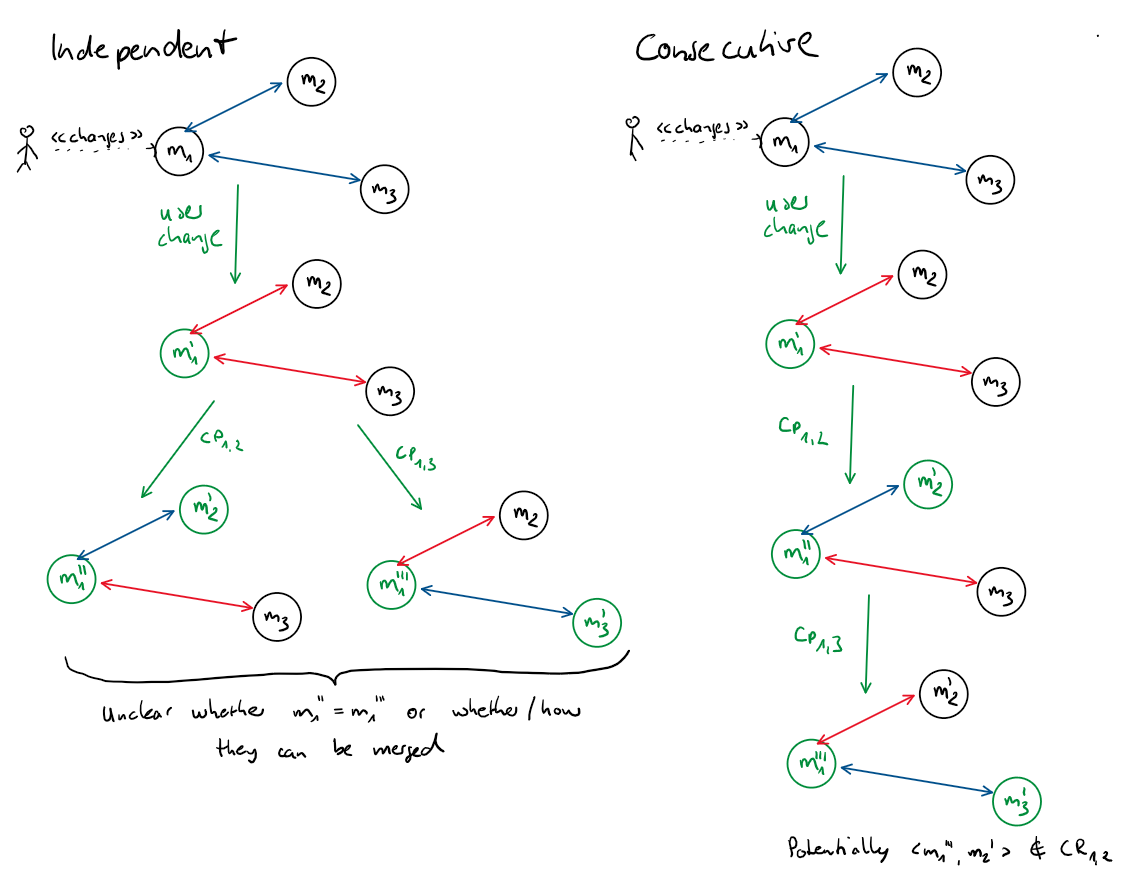
\includegraphics[width=\textwidth]{figures/correctness/notion/concurrent_consecutive_execution.png}
    \caption[Execution alternatives of consistency preservation rules]{Scenarios for independently executing consistency preservation rules on input models and consecutively executing them on the results of other rules.}
    \label{fig:correctness:concurrent_consecutive_execution}
\end{figure}

\mnote{Unification and orchestration necessary due to conflicting sequences}
The examples for the two strategies of executing \glspl{consistency preservation rule} are depicted in \autoref{fig:correctness:concurrent_consecutive_execution}. 
Even if \glspl{consistency preservation rule} were supposed to only modify one model instead of two, like in the examples, the same problems of unification and orchestration would occur as soon as there are two sequences of \glspl{consistency preservation rule} that change the same models.

\mnote{Benefits of consecutive execution}
In our work, we follow the approach of orchestrating and consecutively executing \glspl{consistency preservation rule}.
The benefits of this approach are twofold. First, there is no additional logic required for unifying the changes performed by independently executed \glspl{consistency preservation rule}. 
Second, the unification may deliver a model that is not consistent to any of the \glspl{consistency relation} anymore, whereas consecutive execution at least gives the guarantee that the models are consistent to the last applied \gls{consistency preservation rule}.
With this approach, the preservation rules can \enquote{negotiate} a solution by reacting to the changes the others performed.

\begin{remark} 
\mnote{Monolithic notions are degraded modular ones}
Finally, every monolithic notion of consistency and its preservation can be considered a special case of a modular notion. Having only one consistency relation and one function that preserves it degrades the problem by making the necessity to perform an orchestration of functions obsolete.
\end{remark}

\mnote{Different realization options for consistency preservation rules}
For now, the introduced \glspl{consistency preservation rule} can be any kind of functions that return consistent models. 
Their realization may, for example, be transformations that define how to react to certain changes for restoring consistency, or constraint solvers that find consistent models by solving consistency constraints. 
We do not yet need to consider how these functions are realized to derive consistent models, although, later, we will focus on transformation-based approaches.


\subsection{Declarative and Imperative Consistency Specifications}

\begin{figure}
    \centering
    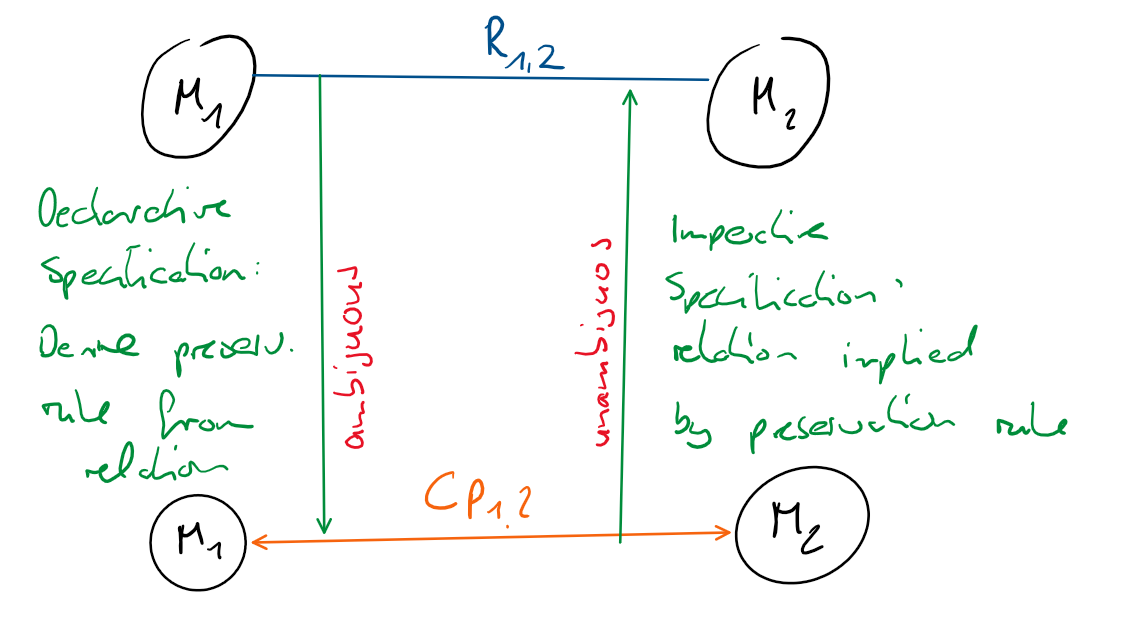
\includegraphics[width=0.7\textwidth]{figures/correctness/notion/declarative_imperative}
    \caption[Declarative and imperative consistency specification]{Declarative and imperative specification of consistency relations and consistency preservation rules}
    \label{fig:correctness:declarative_imperative}
\end{figure}

\mnote{Only define relation \emph{or} function}
We discussed that consistency preservation can be considered as functions, called \glspl{consistency preservation rule}, that preserve consistency according to some relations.
%In practice, consistency preservation is usually specified by means of transformations.
In practice, however, one will usually not specify both the \gls{consistency relation} itself and also the \gls{consistency preservation rule} that preserves it.
Instead, usually one artifact is given and the other is implied or derived.
This leads to the two approaches of \emph{declarative} and \emph{imperative} consistency specifications, depending on whether the specification defines \emph{how} consistency is achieved.
The relation between the two approaches and \glspl{consistency relation} and \glspl{consistency preservation rule} is depicted in \autoref{fig:correctness:declarative_imperative}.

\mnote{Ambiguity in deriving rules from relations}
As a first option, a developer may only define relations that specifies consistency. Functions that preserve these relations can be derived from that.
This is called a \emph{declarative} specification, because it only declares when models are consistent but \emph{how} consistency is achieved.
In general, there is not only a single option how this function can look like.
It can, for example, calculate the result with minimal differences to the input, according to some defined metrics.
Or, especially if there is an intensional specification of that relation, the approach may consider the type of input change and calculate an appropriate change according to the constraints in the intensional specification.
This is the approach that is followed by many declarative transformation languages, such as \gls{QVTR}, or \glspl{TGG}.

\mnote{Relations are induced by fixed-points of functions}
As a second option, a developer can define \glspl{consistency preservation rule}.
These functions imply the underlying \glspl{consistency relation} that they preserve.
Given a function $\function{Cp}$, the relation is implied by its fixed-points: $\consistencyrelation{R}{} = \setted{\modelset{m} \mid \function{Cp}(\modelset{m}) = \modelset{m}}$.
If a function preserving consistency does not perform any changes, the models are, by definition, consistent.
This is called a \emph{imperative} specification, because it declares \emph{how} consistency can be achieved.
Such an approach is followed by many imperative transformation languages, such as \gls{QVTO} or \gls{VIATRA}.


\subsection{Artifacts in Consistency Preservation}

\mnote{Four artifacts for general consistency preservation}
We have discussed that consistency can be considered in a monolithic or modular way. We have, however, also mentioned that the monolithic case can be considered as a special case of the modular one.
For the general case, we thus know from the previous considerations that in a consistency preservation process at least specification that define consistency, called \emph{\glspl{consistency relation}}, functions that preserve consistency, called \emph{\glspl{consistency preservation rule}}, and a function for orchestrating the functions, in the following called \emph{\gls{orchestration function}}, are necessary. Finally, we also need a function that applies the \glspl{consistency preservation rule} in the order that is determined by the orchestration function, which we call the \emph{\gls{application function}}.
To summarize, we consider the following artifacts necessary to handle consistency preservation:
\begin{properdescription}
    \item[\Glspl{consistency relation}:] Binary (or in general n-ary) relations that specify when models are to be considered consistent.
    \item[\Glspl{consistency preservation rule}:] Functions that that restore consistency for a pair (or in general set) of models after they were modified to an inconsistent state.
    \item[\Gls{orchestration function}:] A function that determined in which order the consistency preservation rules have to be executed when the models became inconsistent.
    \item[\Gls{application function}:] A function that is able to apply the consistency preservation rules in the order determined by the orchestration function. 
\end{properdescription}

\mnote{Distinction between orchestration and application}
We explicitly distinguish the orchestration and the application to be able to make more fine-grained statements about the responsibilities for the orchestration and its actual execution.
The process is depicted in \autoref{fig:correctness:execution_process}. Given models that are consistent according to some consistency relations and changes to them that lead to inconsistencies, the orchestration function delivers an order of consistency preservation rules, which is used to parametrize the application function that executes these rules in the given order.
The result is, in the best case, a set of models that is consistent to the relations again.
However, we will see that this is not always possible. Thus, we will especially discuss relevant properties of the artifacts, such as correctness and optimality that reflect how and when this process can be executed successfully.

\begin{figure}
    \centering
    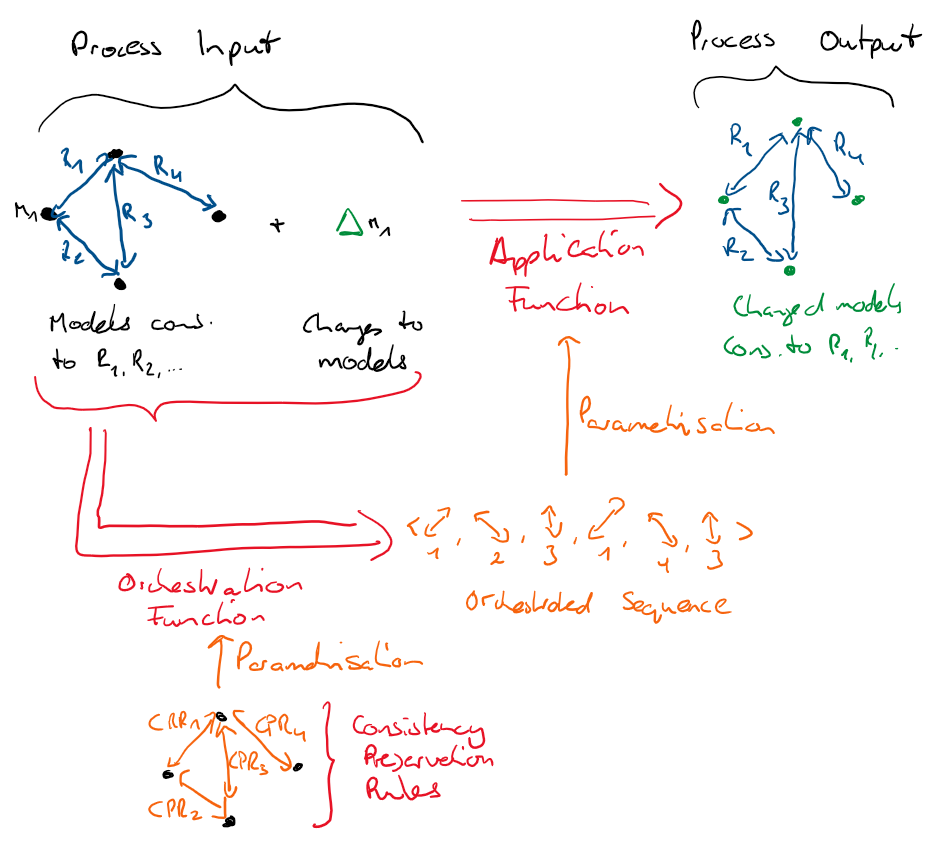
\includegraphics[width=\textwidth]{figures/correctness/notion/execution_process.png}
    \caption[Modular consistency specification execution process and artifacts]{Execution process and artifacts for a modular consistency specification}
    \label{fig:correctness:execution_process}
\end{figure}

